\documentclass[a4paper]{article}

% Algorithms
\usepackage[linesnumbered,vlined,ruled,commentsnumbered]{algorithm2e}

% Babel
\usepackage[english]{babel}

% Code writing
	%\usepackage[procnames]{listings}

% Font
\usepackage[utf8]{inputenc}
\usepackage[T1]{fontenc}
\usepackage[fleqn]{amsmath}
\usepackage{amssymb,amsthm,amsfonts}
\usepackage{mathtools}
\usepackage{eucal}
\usepackage{textcomp}
\usepackage{dsfont}
\usepackage{bbm}
%\usepackage{newunicodechar}

% Footnote


% Hyperref
\usepackage[hyphens]{url}
\usepackage{cite}
\usepackage{hyperref}
\usepackage{nameref}

% Images
\usepackage[pdftex]{graphicx}
%\usepackage{subfigure}
\usepackage{subfig}
\usepackage{eso-pic}
\usepackage{caption}
\usepackage{wrapfig}
\usepackage{float}

% List
\usepackage{enumerate}

% SI units
\usepackage{siunitx}

% Standalone
\usepackage[subpreambles=true]{standalone}
\usepackage{import}

% Tables
\usepackage{tabularx}
\usepackage{booktabs}
\usepackage{multirow}

% TiKz and graphs
\usepackage{pgf,tikz,pgfplots}
% \usepackage{gnuplottex}
\usepackage{bm}
\usepackage{relsize}
\usepackage{tikz-3dplot}
\usepackage[compat=1.1.0]{tikz-feynman}
\usepackage{circuitikz}
\pgfplotsset{compat=1.16}

% Typeset
\usepackage[top=2cm,bottom=2cm,left=2cm,right=2cm]{geometry}
\usepackage{fancyhdr}
\usepackage{indentfirst}
\usepackage{titlesec}
\usepackage{setspace}
\usepackage{xspace}
% \usepackage{parskip}  % Elimina il separatore a inizio paragrafo
\usepackage{afterpage}
\usepackage{comment}

%Python
\usepackage{xcolor}
\usepackage{listings}
\usepackage{framed}

%Per scrivere matrice identità
%Per semplificazione formule
\usepackage{cancel}

% Others
\usepackage{empheq}
\usepackage{soul}
%Evidenziare testo con mdframed
\usepackage{mdframed}
%Note a margine
\usepackage{marginnote}
\usepackage{mparhack}
%Display data
\usepackage{datetime}
%Physics
\usepackage{physics}

\usepackage[many,most,theorems]{tcolorbox}

%Geometry
\makeatletter
\renewcommand{\@marginparreset}{%
  \reset@font\small
  \raggedright
  \slshape
  \@setminipage
}
\makeatother

\captionsetup[table]{font=small,labelfont={bf},skip=10pt}
\captionsetup[figure]{font=small,labelfont={bf},skip=10pt}


%link ipertestuale per indice
\hypersetup{
	colorlinks=false,
	linkcolor=black,
	filecolor=blue,
	citecolor = blue,
	urlcolor=blue,
	}

%%%%%indent%%%
\setlength{\parindent}{0pt}
\setlength{\parskip}{0pt}
\setlength{\mathindent}{1.5em}




%Python in latex
\definecolor{codegreen}{rgb}{0,0.6,0}
\definecolor{codegray}{rgb}{0.5,0.5,0.5}
\definecolor{codepurple}{rgb}{0.58,0,0.82}
\definecolor{backcolour}{rgb}{0.95,0.95,0.92}
\definecolor{commentcolour}{rgb}{0.43,0.63,0.65}

\definecolor{shadecolor}{rgb}{0.93, 0.93, 0.93}
\definecolor{darkgreen}{rgb}{0.0, 0.4, 0.0}
\definecolor{darkred}{rgb}{0.8, 0.0, 0.0}
\definecolor{violet}{rgb}{0.55, 0.0, 0.55}

%\lstdefinestyle{mystyle}{ %Stile python code
%    backgroundcolor=\color{shadecolor},
%    commentstyle=\color{commentcolour},
%    keywordstyle=\color{darkgreen},
%    numberstyle=\tiny\color{codegray},
%    stringstyle=\color{darkred},
%    basicstyle=\ttfamily\footnotesize,
%    breakatwhitespace=false,
%    breaklines=true,
%    captionpos=b,
%    keepspaces=true,
%    numbers=left,
%    numbersep=5pt,
%    showspaces=false,
%    showstringspaces=false,
%    showtabs=false,
%    tabsize=2
%}
%
%\lstset{style=mystyle}

% Derivatives
\renewcommand{\d}[0]{\mathrm{d}}
\newcommand{\dev}[2]{\displaystyle \frac{\d #1}{\d #2}}
\newcommand{\pdev}[2]{\displaystyle \frac{\partial #1}{\partial #2}}
\newcommand{\ndev}[3]{\displaystyle \frac{\d^{#3} #1}{\d #2^{#3} } }
\newcommand{\npdev}[3]{\displaystyle \frac{\partial^{#3} #1}{\partial #2^{#3} } }

%% Math operators
\DeclareMathOperator{\arctanh}{arctanh}
\DeclareMathOperator{\sign}{sign}

%% Norms
\newcommand{\absvec}[1]{| \vec{#1} |}
\newcommand{\normvec}[1]{|\!| #1 |\!|}

%% User defined commands
\newcommand{\mathcolorbox}[2]{\colorbox{#1}{$\displaystyle #2$}}
\newcommand{\hlfancy}[2]{\sethlcolor{#1}\hl{#2}}

%% User defined math commands
\newcommand{\R}{\mathbb{R}}
\newcommand{\C}{\mathbb{C}}
\newcommand{\vmed}[1]{\left \langle #1 \right \rangle}
\newcommand{\vmedvec}[1]{\langle #1 \rangle}
\newcommand{\id}{\mathbbm{1}}
\newcommand{\floor}[1]{\left \lfloor #1 \right \rfloor}
\newcommand{\ceil}[1]{\left \lceil #1 \right \rceil}
\renewcommand{\exp}[1]{\operatorname{e}^{#1}}
\renewcommand{\H}[0]{\operatorname{H}}
\renewcommand{\Re}[1]{\operatorname{\mathbb{R}e}\left[ #1 \right]}
\renewcommand{\Im}[1]{\operatorname{\mathbb{I}m}\left[ #1 \right]}

\newtcbtheorem{theorem}{Theorem}{ % frame stuff
    boxrule = 1pt,
    breakable,
    enhanced,
    frame empty,
    interior style= {orange!20},
    %interior empty,
    colframe=black,
    borderline ={1pt}{0pt}{black},
    left=0.2cm,
    % title stuff
    attach boxed title to top left={yshift=-2mm,xshift=0mm},
    coltitle=black,
    fonttitle=\bfseries,
    colbacktitle=white,
    fontupper=\slshape,
    boxed title style={boxrule=1pt,sharp corners}}{theorem}

\newtcbtheorem{corollary}{Corollary}{ % frame stuff
    boxrule = 1pt,
    breakable,
    enhanced,
    frame empty,
    interior style= {orange!20},
    %interior empty,
    colframe=black,
    borderline ={1pt}{0pt}{black},
    left=0.2cm,
    % title stuff
    attach boxed title to top left={yshift=-2mm,xshift=0mm},
    coltitle=black,
    fonttitle=\bfseries,
    colbacktitle=white,
    fontupper=\slshape,
    boxed title style={boxrule=1pt,sharp corners}}{corollary}

\newtcbtheorem{lemma}{Lemma}{ % frame stuff
    boxrule = 1pt,
    breakable,
    enhanced,
    frame empty,
    interior style= {orange!20},
    %interior empty,
    colframe=black,
    borderline ={1pt}{0pt}{black},
    left=0.2cm,
    % title stuff
    attach boxed title to top left={yshift=-2mm,xshift=0mm},
    coltitle=black,
    fonttitle=\bfseries,
    colbacktitle=white,
    fontupper=\slshape,
    boxed title style={boxrule=1pt,sharp corners}}{lemma}


%%%%%%%%%%%%%%%%%%%%Definition%%%%%%%%%%%%%%%%%


\newtcbtheorem{definition}{Definition}{ % frame stuff
    boxrule = 1pt,
    breakable,
    enhanced,
    frame empty,
    interior style= {blue!10},
    %interior empty,
    colframe=black,
    borderline ={1pt}{0pt}{black},
    left=0.2cm,
    % title stuff
    attach boxed title to top left={yshift=-2mm,xshift=0mm},
    coltitle=black,
    fonttitle=\bfseries,
    colbacktitle=white,
    boxed title style={boxrule=1pt,sharp corners}}{definition}


%\theoremstyle{definition}
%\newtheorem{definition}{Definition}%[section]



%%%%%%%%%%%%%%%%%%%%Exercise and example%%%%%%%%%%%%%%%%%

\newtcbtheorem{exercise}{Exercise}{ % frame stuff
    boxrule = 1pt,
    breakable,
    enhanced,
    frame empty,
    interior style= {blue!6},
    %interior empty,
    colframe=black,
    borderline ={1pt}{0pt}{black},
    left=0.2cm,
    % title stuff
    attach boxed title to top left={yshift=-2mm,xshift=0mm},
    coltitle=black,
    fonttitle=\bfseries,
    colbacktitle=white,
    boxed title style={boxrule=1pt,sharp corners}}{exercise}

\newtcbtheorem{example}{Example}{ % frame stuff
    boxrule = 1pt,
    enhanced,
    frame empty,
    interior style= {green!6},%{left color=yellow!70,right color=green!70},
    %interior empty,
    colframe=black,
    borderline ={1pt}{0pt}{black},
    breakable,
    left=0.2cm,
    % title stuff
    attach boxed title to top left={yshift=-2mm,xshift=0mm},
    coltitle=black,
    fonttitle=\bfseries,
    colbacktitle=white,
    boxed title style={boxrule=1pt,sharp corners}}{example}

%\newtheorem{exercise}{Exercise}
%\newtheorem{example}{Example}

%%%%%%%%%%%%%%%%%%%%%%%%%%%%%%%%%%%

\theoremstyle{remark}
\newtheorem*{remark}{Remark}
\newtheorem{observation}{Observation}
%Evidenziare testo
\newtheorem*{solution}{Solution}

\newcommand\mybox[1]{%
  \fbox{\begin{minipage}{0.9\textwidth}#1\end{minipage}}}

  %Spiegazioni/verifiche
\newenvironment{greenbox}{\begin{mdframed}[hidealllines=true,backgroundcolor=green!20,innerleftmargin=3pt,innerrightmargin=3pt,innertopmargin=3pt,innerbottommargin=3pt]}{\end{mdframed}}

\newenvironment{bluebox}{\begin{mdframed}[hidealllines=true,backgroundcolor=blue!10,innerleftmargin=3pt,innerrightmargin=3pt,innertopmargin=3pt,innerbottommargin=3pt]}{\end{mdframed}}

\newenvironment{yellowbox}{\begin{mdframed}[hidealllines=true,backgroundcolor=yellow!20,innerleftmargin=3pt,innerrightmargin=3pt,innertopmargin=3pt,innerbottommargin=3pt]}{\end{mdframed}}

\newenvironment{redbox}{\begin{mdframed}[hidealllines=true,backgroundcolor=red!20,innerleftmargin=3pt,innerrightmargin=3pt,innertopmargin=3pt,innerbottommargin=3pt]}{\end{mdframed}}

\newenvironment{orangebox}{\begin{mdframed}[hidealllines=true,backgroundcolor=orange!20,innerleftmargin=3pt,innerrightmargin=3pt,innertopmargin=3pt,innerbottommargin=3pt]}{\end{mdframed}}

%emph equation
\newcommand*\myyellowbox[1]{%
  \colorbox{yellow!40}{\hspace{1em}#1\hspace{1em}}}

\newcommand*\mygreenbox[1]{%
  \colorbox{green!20}{\hspace{1em}#1\hspace{1em}}}


%%%%%%%%%%PROOF%%%%%%%%%%%%%%%%%%%%%%%%%%%%%
\usepackage{xpatch}
\xpatchcmd{\proof}{\itshape}{\normalfont\proofnamefont}{}{}
\newcommand{\proofnamefont}{\bfseries}
\renewcommand\qedsymbol{$\blacksquare$}


\newcommand\Warning{%
	\makebox[1.4em][c]{%
		\makebox[0pt][c]{\raisebox{.1em}{\small!}}%
		\makebox[0pt][c]{\color{red}\Large$\bigtriangleup$}
	}
}%

\definecolor{mygreen}{rgb}{0,0.6,0}
\definecolor{mygray}{rgb}{0.5,0.5,0.5}
\definecolor{mymauve}{rgb}{0.58,0,0.82}
\lstset{
	basicstyle=\ttfamily\footnotesize,        % the size of the fonts that are used for the code
	breakatwhitespace=false,                  % sets if automatic breaks should only happen at whitespace
	breaklines=false,                         % sets automatic line breaking
	captionpos=b,                             % sets the caption-position to bottom
	commentstyle=\color{mygreen},             % comment style
	extendedchars=true,                       % lets you use non-ASCII characters; for 8-bits encodings only, does not work with UTF-8
	keepspaces=true,                          % keeps spaces in text, useful for keeping indentation of code (possibly needs columns=flexible)
	keywordstyle=\color{blue},                % keyword style
	language=[95]Fortran,                     % the language of the code
	numbers=left,                             % where to put the line-numbers; possible values are (none, left, right)
	numbersep=5pt,                            % how far the line-numbers are from the code
	numberstyle=\tiny\color{mygray},          % the style that is used for the line-numbers
	rulecolor=\color{black},                  % if not set, the frame-color may be changed on line-breaks within not-black text (e.g. comments (green here))
	showspaces=false,                         % show spaces everywhere adding particular underscores; it overrides 'showstringspaces'
	showstringspaces=false,                   % underline spaces within strings only
	showtabs=false,                           % show tabs within strings adding particular underscores
	stepnumber=1,                             % the step between two line-numbers. If it's 1, each line will be numbered
	stringstyle=\color{mymauve},              % string literal style
	tabsize=4,                                % sets default tabsize to 2 spaces
	title=\lstname                            % show the filename of files
}



\title{\textbf{\huge Quantum Information and Computing}\\Week 1 assignment}
\author{Ardino Rocco\\Mat. 1231629\\\href{mailto:rocco.ardino@studenti.unipd.it}{rocco.ardino@studenti.unipd.it}}
\date{\today}





\begin{document}

\maketitle
\vspace{1cm}


\section*{Exercise 1}
The setup of the workspace was accomplished without any trouble. After, creating a working directory, inside this the following code for a test job is written:

\begin{lstlisting}[label={lst:01_ex1_1},caption={Test job submitted.}]
! 01_ex1.f90

program setup

	implicit none

	print*, "Hello World!"

end program
\end{lstlisting}

After accessing to spiro.fisica.unipd.it through \texttt{ssh} protocol, the test job is compiled through gfortran compiler and correctly submitted and executed.





\section*{Exercise 2}
The first sum of the numbers \( 1 \) and \( 2000000 \) is performed using integers of 2 bytes and then of 4 bytes. In the first case, there is evidence of overflow since the result is not correct (\( -31615 \)). In the second case, the operation returns the correct result.

The second sum of the numbers \( \pi \cdot 10^{32} \) and \( \sqrt{2} \cdot 10^{21} \) is performed using floating points of 4 bytes and then of 8 bytes. The first operation returns the correct result up to the seventh significant digit in comparison to the second operation, which is considered much more accurate for the greater number of bytes involved.





\section*{Exercise 3}
Several implementations of matrix matrix multiplication are possible, depending on the order of the loops needed for the purpose. The two implementations for this report are given in Listings \ref{lst:01_ex3_1} and \ref{lst:01_ex3_2}.

\begin{lstlisting}[label={lst:01_ex3_1},caption={First implementation of matrix matrix multiplication.}]
! matrix matrix multiplication by column
function matmul_col(mat1, mat2) result(mat3)
	integer*2 :: ii, jj, kk
	integer*2 :: N, M, L
	real*4, dimension(:,:) :: mat1, mat2
	real*4, dimension(size(mat1, 1),size(mat2, 2)) :: mat3

	N = size(mat1, 1)
	M = size(mat1, 2)
	L = size(mat2, 2)

	do jj=1,M
		do kk=1,L
			do ii=1,N
				mat3(ii,jj) = mat3(ii,jj) + mat1(ii,kk)*mat2(kk,jj)
			end do
		end do
	end do
end function
\end{lstlisting}

\begin{lstlisting}[label={lst:01_ex3_2},caption={Second implementation of matrix matrix multiplication.}]
! matrix matrix multiplication by row
function matmul_row(mat1, mat2) result(mat3)
	integer*2 :: ii, jj, kk
	integer*2 :: N, M, L
	real*4, dimension(:,:) :: mat1, mat2
	real*4, dimension(size(mat1, 1),size(mat2, 2)) :: mat3

	N = size(mat1, 1)
	M = size(mat1, 2)
	L = size(mat2, 2)

	do ii=1,N
		do kk=1,L
			do jj=1,M
				mat3(ii,jj) = mat3(ii,jj) + mat1(ii,kk)*mat2(kk,jj)
			end do
		end do
	end do
end function
\end{lstlisting}

Their performances are monitored for \( n \times n \) matrices through the function \texttt{CPU\_TIME} and for different values of \( n \). The results are showed in Figure \ref{fig:01_ex3_1}. It is possible to see how the first implementation is slightly faster than the second one and how the two user implementations are much slower than the intrinsic one. The first fact is due to the way fortran stores variables in memory when dealing with arrays. In fact, this is done by columns, so the first implementation is faster since the inner loop is over consecutive elements in memory. The second fact is due to a different implementation highly optimized using state of the art algorithms.

\begin{figure}[!h]
	\centering
	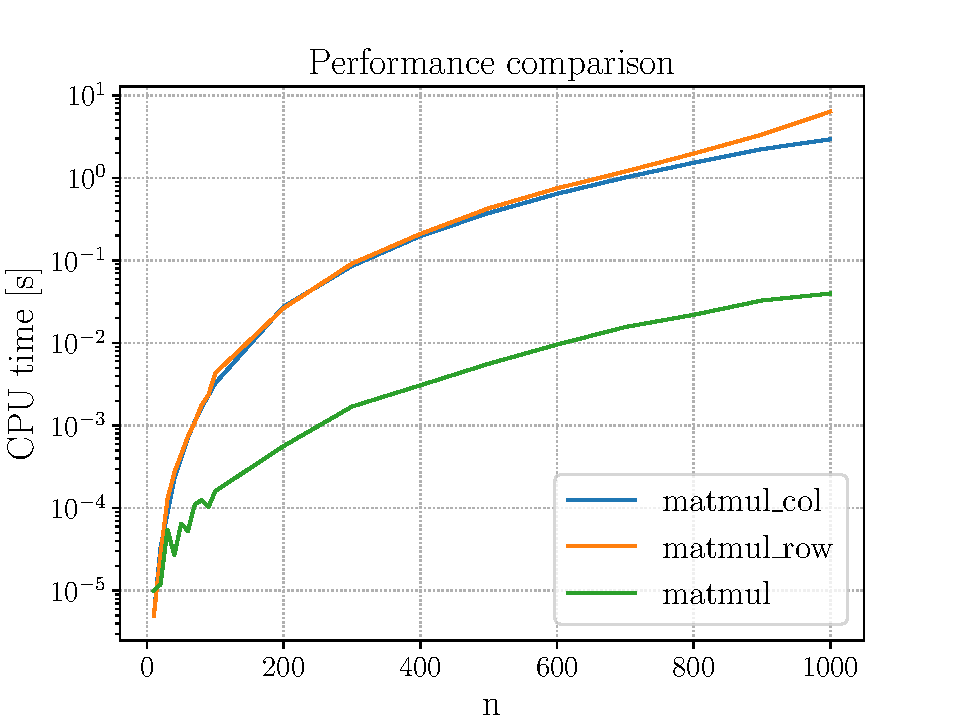
\includegraphics[width=0.5\textwidth]{images/01_ex3_performance.pdf}
	\caption{\label{fig:01_ex3_1} Performances of the two implementations and of the intrinsic function depending on the matrix size \( n \).}
\end{figure}

Another test on the execution speed is done by applying different optimization flags, listed in Table \ref{tab:01_ex3_1}. The same analysis done before is performed for every implementation and for every optimization flag. Again, the results are plotted in order to compare how the different flags affect the execution time of the matrix matrix multiplication. The plots are showed in Figure \ref{fig:01_ex3_2}.

\begin{table}[!h]
	\centering
	\begin{tabular}{ccccc}
		\toprule
		Flag	&	Exec. time	&	Code size	&	Mem. usage	&	Compile time	\\
		\midrule
		\texttt{-O0}	&	\( + \) 	&	\( + \)	&	\( - \)	&	\( - \)  	\\
		\texttt{-O1}	&	\( - \) 	&	\( - \)	&	\( + \)	&	\( + \)  	\\
		\texttt{-O2}	&	\( -- \)	&	       	&	\( + \)	&	\( ++ \) 	\\
		\texttt{-O3}	&	\( --- \)	&	       	&	\( + \)	&	\( +++ \)	\\
		\texttt{-Ofast}	&	\( --- \)	&	       	&	\( + \)	&	\( +++ \)	\\
		\bottomrule
	\end{tabular}
	\caption{Optimization flags effects.}
	\label{tab:01_ex3_1}
\end{table}

\begin{figure}[H]
	\centering
	\begin{minipage}[t]{0.32\linewidth}
		\centering
		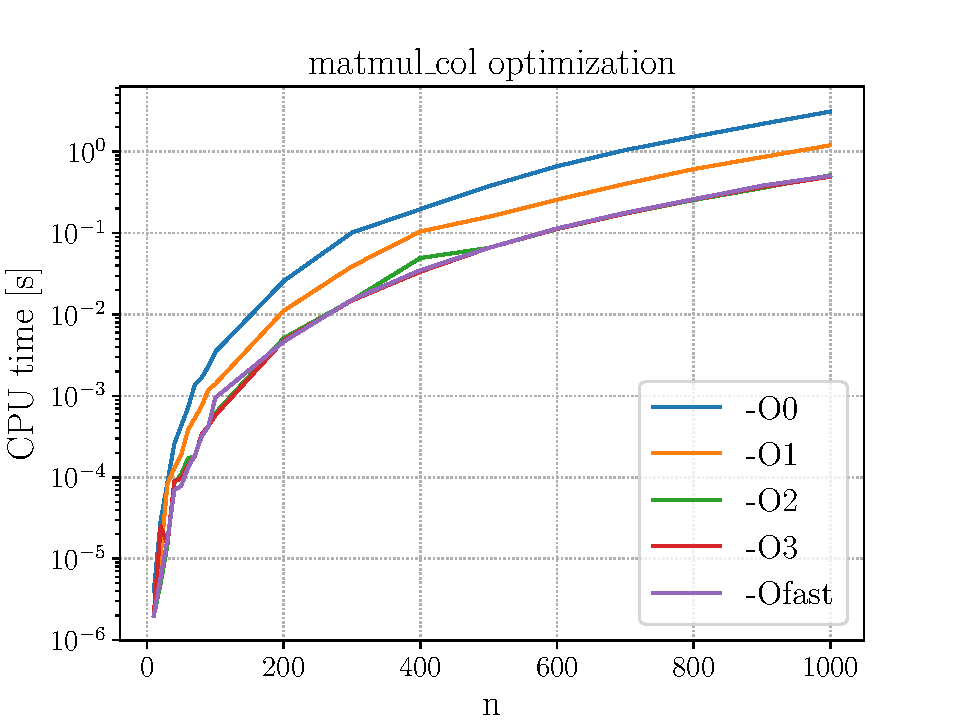
\includegraphics[width=1\textwidth]{images/01_ex3_matmul_col_O.pdf}
	\end{minipage}
	\begin{minipage}[t]{0.32\linewidth}
		\centering
		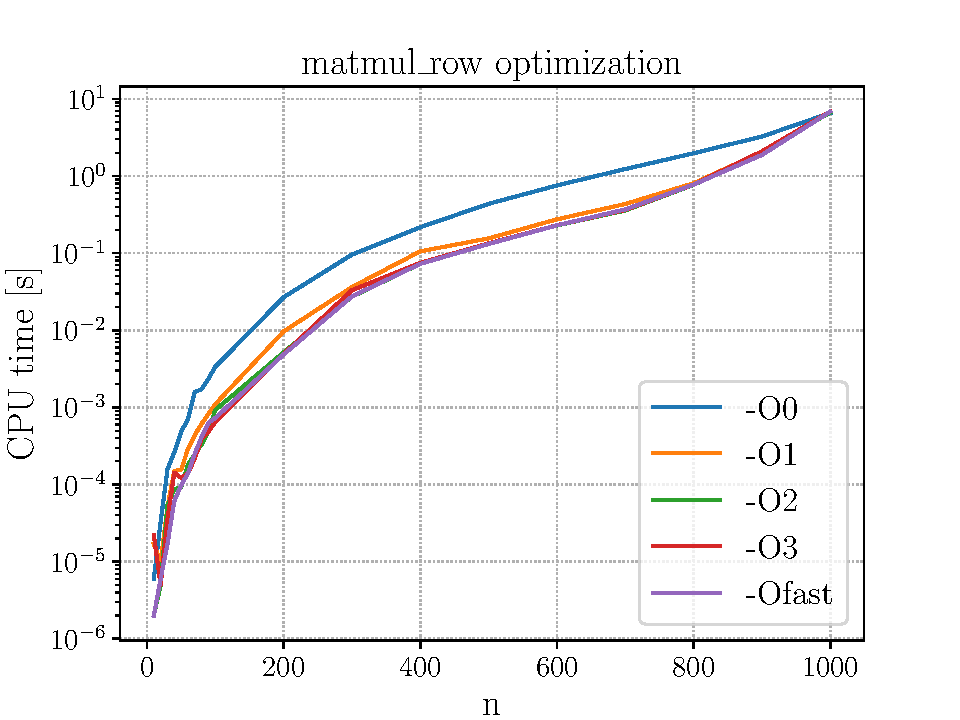
\includegraphics[width=1\textwidth]{images/01_ex3_matmul_row_O.pdf}
	\end{minipage}
	\begin{minipage}[t]{0.32\linewidth}
		\centering
		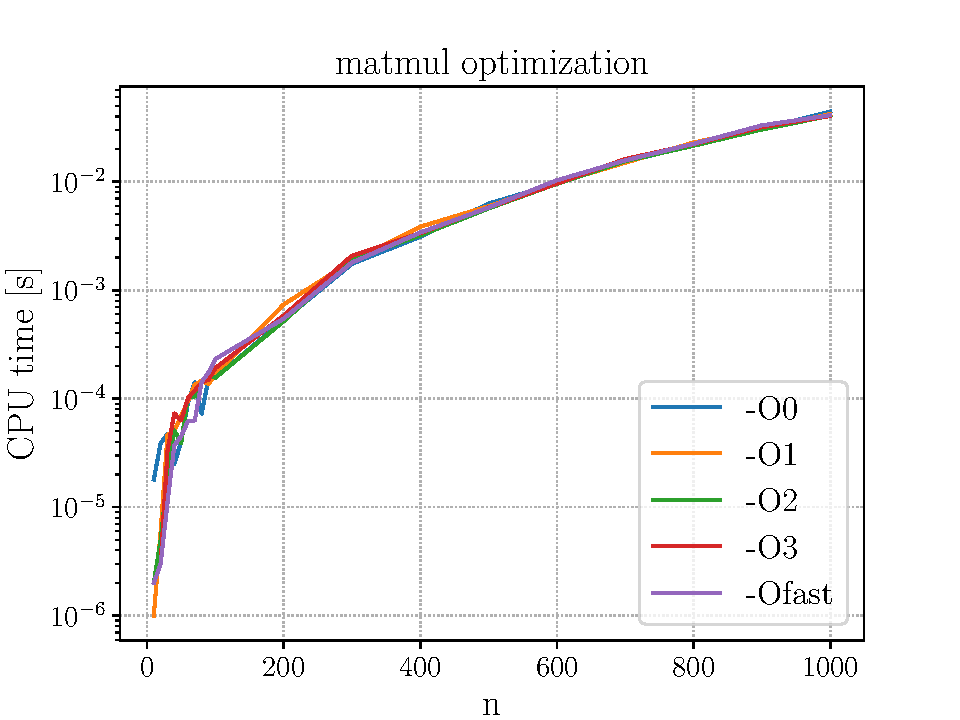
\includegraphics[width=1\textwidth]{images/01_ex3_matmul_O.pdf}
	\end{minipage}
	\caption{\label{fig:01_ex3_2} Left: execution time for the first implementation for several optimization flags. Center: execution time for the second implementation for several optimization flags. Right: execution time for the intrinsic function for several optimization flags.}
\end{figure}

\end{document}
